\begin{frame}{Random Forests -- method summary}

% \maketag{SUPERVISED} 
\maketag{regression} \maketag{classification}
\maketag{NONPARAMETRIC} \maketag[50]{BLACK-BOX} \maketag{FEATURE SELECTION}

\medskip

\highlight{General idea} 
\begin{itemize}
  \item \textbf{Bagging ensemble} of $M$ tree \textbf{base learners} fitted on \textbf{bootstrap} data samples\\
   ~~ $\Rightarrow$ Reduce \textbf{variance} by ensembling while slightly increasing \textbf{bias} by bootstrapping  
   \begin{itemize}
    \item Use unstable, \textbf{high-variance} base learners by letting trees grow to full size
    \item Promoting \textbf{decorrelation} by random subset of candidate features for each split
  \end{itemize}
  \item \textbf{Predict} via averaging (regression) or majority vote (classification) of base learners
\end{itemize}

\medskip

\highlight{Hypothesis space} ~~
$\Hspace = \left\{ \fx: \fx = \frac{1}{M} \sum\limits_{m = 1}^M 
\sum\limits_{t = 1}^{T^{[m]}} 
c_t^{[m]} \I(\xv \in Q_t^{[m]}) \right\}$

%\medskip

\begin{minipage}[b]{0.65\textwidth}
  % FIGURE SOURCE: https://docs.google.com/presentation/d/1xodP6ayu1Gay6mMKgzVWYEFmSoeG5kNuqsaTkFFmd78  /edit
  \centering
  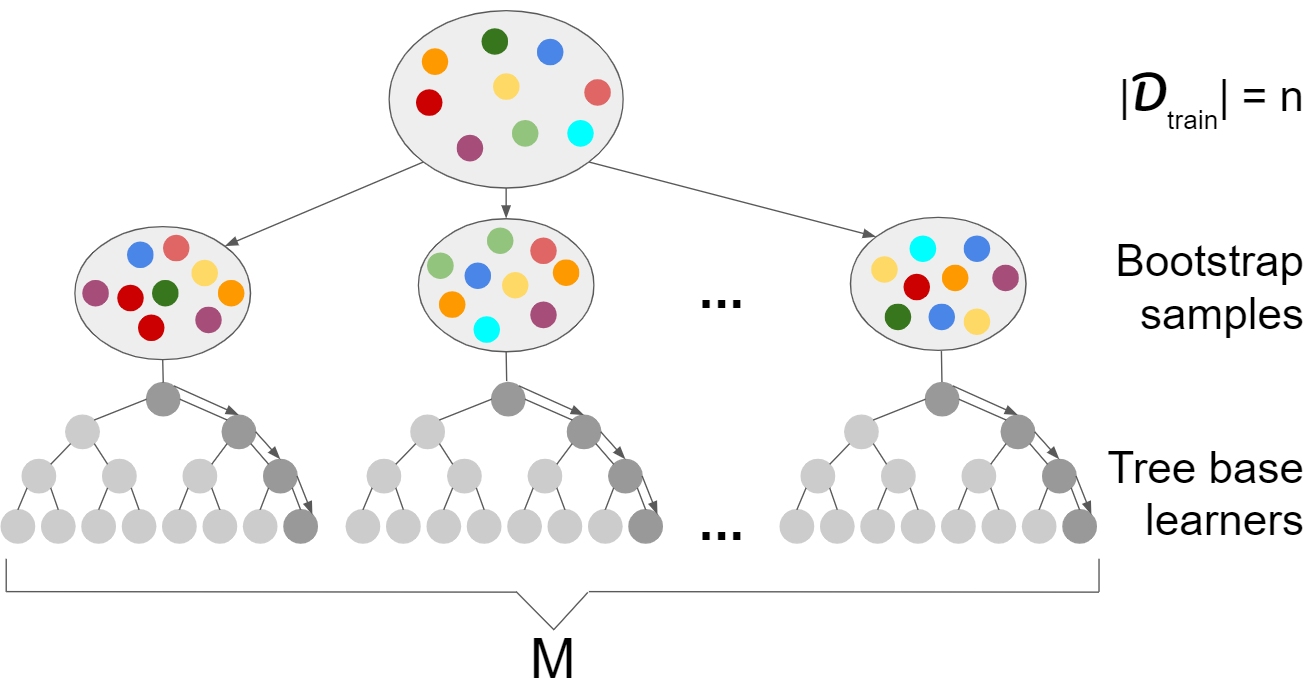
\includegraphics[width=0.6\textwidth]{figure/rf-bagging} \\
  \tiny Schematic depiction of bagging process
\end{minipage}%
\begin{minipage}[b]{0.35\textwidth}
\centering
  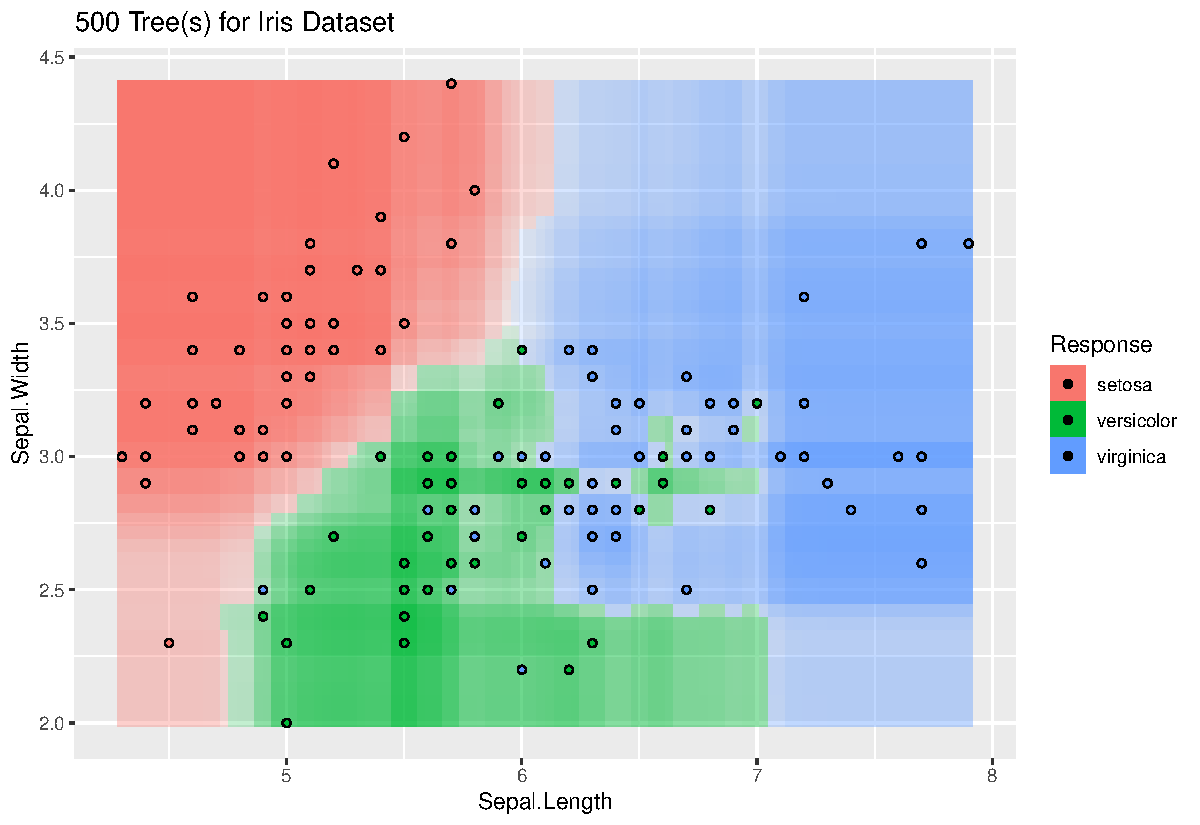
\includegraphics[width=0.9\textwidth]{
  ../slides/forests/figure/cart_forest_intro_3} \\
  \tiny Prediction surface for \texttt{iris} data with 500-tree ensemble
\end{minipage}

\end{frame}

% ------------------------------------------------------------------------------

\begin{frame}{Random Forests -- method summary}

\highlight{Empirical risk \& Optimization} ~~ Just like tree base learners

\medskip

\highlight{Out-of-bag (OOB) error}
\begin{itemize}
  \item Ensemble prediction for obs. outside individual trees' bootstrap training sample $\Rightarrow$ unseen test sample
  \item Use resulting loss as unbiased estimate of \textbf{generalization error}
  \item Mainly useful for tuning and less for model comparison as we usually compare all models uniformly by CV
\end{itemize}

\medskip

\highlight{Feature importance}

\begin{itemize}
  \item Based on \textbf{improvement in split criterion:} aggregate improvements 
  by all splits using $j$-th feature
  \item Based on \textbf{permutation:} permute $j$-th feature in 
  OOB observations and compute impact on OOB error
\end{itemize}

\medskip

\highlight{Hyperparameters}

\begin{itemize}
  \item \textbf{Ensemble size}, i.e., number of trees
  \item \textbf{Complexity} of base learners, e.g., tree depth, min-split, min-leaf-size
  \item \textbf{Number of split candidates}, i.e., number of features to be considered at each split \\
  $\Rightarrow$ frequently used heuristics with total of $p$ features: 
  $\left \lfloor{\sqrt{p}}\right \rfloor$ for classification, $\left \lfloor{p/3}\right \rfloor$ for regression
\end{itemize}

% \highlight{Runtime behavior} ~~
% $\mathcal{O}(M \cdot n^2 \cdot p)$ for $M$ trees, $n$ observations and $p$ 
% features
  
\end{frame}


% ------------------------------------------------------------------------------

\begin{frame}{Random Forests -- Implementation \& Practical hints}

\highlight{Extremely Randomized Trees}
\begin{itemize}
    \item Variance of trees can be further increased by \textbf{randomizing split points} instead of using the optimal one
    \item Alternatively consider $k$ random splits and pick the best one according to impurity 
\end{itemize}

\medskip

\highlight{Tuning} 
\begin{itemize}
    \item \textbf{Ensemble size} should not be tuned as it only decreases variance $\longrightarrow$ choose sufficiently large ensemble
    \item While default values for \textbf{number of split points} is often good, tuning it can still improve performance
    \item Tuning the \textbf{minimum samples in leafs} and \textbf{minimum samples for splitting} can be benificial but no huge performance increases are to be expected 
\end{itemize}

\medskip

\highlight{Implementation}

\begin{itemize}
  \item \textbf{R:} \texttt{mlr3} learners \texttt{LearnerClassifRanger} / 
    \texttt{LearnerRegrRanger}, calling \texttt{ranger::ranger()} as a highly efficient and flexible implementation
  \item \textbf{Python:} \texttt{RandomForestClassifier} / 
  \texttt{RandomForestRegressor} from package \texttt{scikit-learn}
\end{itemize}

\end{frame}

% ------------------------------------------------------------------------------

\begin{frame}{Random Forests -- Pros \& Cons}

\begin{columns}[onlytextwidth]
  \begin{column}{0.5\textwidth}
    \highlight{Advantages}
    \footnotesize
    \begin{itemize}
      \positem Retains most of \textbf{trees'} advantages (e.g., feature selection, feature interactions)
      \positem Fairly \textbf{good predictor}: mitigating base learners' variance through bagging
      \positem Quite \textbf{robust} w.r.t. small changes in data
      \positem Good with \textbf{high-dimensional} data, even in presence of noisy features
      % \positem Applicable to \textbf{unbalanced} data
      \positem Easy to \textbf{parallelize}
      \positem Robust to its hyperparameter configuration
      \positem Intuitive measures of \textbf{feature importance}
    \end{itemize}
  \end{column}
  \begin{column}{0.5\textwidth}
    \highlight{Disadvantages}
    \footnotesize
    \begin{itemize}
      \negitem Loss of individual trees' \textbf{interpretability}
      \negitem Can be suboptimal for \textbf{regression} when extrapolation is needed
      \negitem \textbf{Bias} toward selecting features with many categories (same as CART)
      \negitem Rather large model size and slow inference time for large ensembles
      \negitem Typically inferior in \textbf{performance} to tuned gradient tree boosting.
    \end{itemize}
  \end{column}
\end{columns}

\end{frame}